%%%%%%%%%%%%%%%%%%%%%%%%%%%%%%%%%%%%%%%%%
% FRI Data Science_report LaTeX Template
% Version 1.0 (28/1/2020)
% 
% Jure Demšar (jure.demsar@fri.uni-lj.si)
%
% Based on MicromouseSymp article template by:
% Mathias Legrand (legrand.mathias@gmail.com) 
% With extensive modifications by:
% Antonio Valente (antonio.luis.valente@gmail.com)
%
% License:
% CC BY-NC-SA 3.0 (http://creativecommons.org/licenses/by-nc-sa/3.0/)
%
%%%%%%%%%%%%%%%%%%%%%%%%%%%%%%%%%%%%%%%%%


%----------------------------------------------------------------------------------------
%	PACKAGES AND OTHER DOCUMENT CONFIGURATIONS
%----------------------------------------------------------------------------------------
\documentclass[fleqn,moreauthors,10pt]{ds_report}
\usepackage[english]{babel}

% added this
\usepackage{multirow}
\newcommand{\STAB}[1]{\begin{tabular}{@{}c@{}}#1\end{tabular}}
\usepackage{tabularx}

\graphicspath{{fig/}}




%----------------------------------------------------------------------------------------
%	ARTICLE INFORMATION
%----------------------------------------------------------------------------------------

% Header
\JournalInfo{Natural Language Processing 2023}

% Interim or final report
% \Archive{Second submission report} 
\Archive{Final report} 

% Article title
\PaperTitle{Slovenian Language Assistant for Virtual Conversations (SLAVC)} 

% Authors (student competitors) and their info
\Authors{Luka Škodnik, Robert Jutreša, Valter Hudovernik}

% Advisors
\affiliation{\textit{Advisors: doc. dr. Slavko Žitnik}}

% Keywords
\Keywords{Large Language Models, Machine Translation, Conversational AI, Slovene, Question Answering}
\newcommand{\keywordname}{Keywords}


%----------------------------------------------------------------------------------------
%	ABSTRACT
%----------------------------------------------------------------------------------------

\Abstract{
This report presents the Slovenian Language Assistant for Virtual Conversations (SLAVC), a project developed for the Natural Language Processing course. SLAVC aims to build a conversational agent for the Slovenian language by leveraging large language models (LLMs) and machine translation techniques. The project focuses on translating and processing the OpenAssistant Conversations dataset and adapting transformer models such as T5 and GPT2 for conversation generation. This project demonstrates that utilizing a high-quality dataset and performing translation enables the fine-tuning of conversational models, resulting in the generation of coherent and sometimes even informative responses.
}

%----------------------------------------------------------------------------------------

\begin{document}

% Makes all text pages the same height
\flushbottom 

% Print the title and abstract box
\maketitle 

% Removes page numbering from the first page
\thispagestyle{empty} 

%----------------------------------------------------------------------------------------
%	ARTICLE CONTENTS
%----------------------------------------------------------------------------------------
\section*{Introduction}
	Natural Language Processing (NLP) is an exciting field of Artificial Intelligence that focuses on teaching machines how to understand and respond to human language. 
    In this report, we will discuss our project for the Natural Language Processing course 2022/23, where we aim to develop a Slovenian Conversational Agent called Slovenian Language Assistant for Virtual Conversations  or SLAVC for short.
    % We will provide an overview of our preliminary research, discuss our idea to use a GPT-based model, and explore various data sources that we plan to use to train our model.
    We will provide an overview of our preliminary research, current implementation and explore various data sources that we plan to use and discuss possible models to train or finetune our model.
    % Finally, we will discuss the importance of estimating the amount of data required to train a model effectively.

%------------------------------------------------    
\section*{Related Work}

% Attention & Transformers
%-------------------------
\subsection*{Transformers \& Large Language Models}
Attention \cite{vaswani2017attention} is a key component of transformer models, which are widely used in natural language processing tasks such as language translation and text summarization.
It is also a part of many modern large language models (LLM) that we will use during this project.
In transformer models, attention mechanisms allow the model to focus on the most relevant parts of the input sequence at each step of processing.
This is achieved by assigning weights to each element in the input sequence based on its relevance to the current step.
By doing so, the transformer can capture long-range dependencies between different parts of the input sequence, which is particularly important for language processing. Two notable language models used in this report are T5 \cite{DBLP:journals/corr/abs-1910-10683} and GPT2 \cite{radford2019language}, which we also adapt as conversational agents, due to the pre-training made available by Ulčar and Šikonja \cite{ulčar2023sequence}. 

% SloBERTa
SloBERTa \cite{ulvcar2021sloberta} is a Slovene large language model. It is a large pre-trained masked language model based on the BERT architecture. The authors trained the model on a large corpus of Slovene text and evaluated it on various downstream tasks such as text classification, named entity recognition, and part-of-speech tagging. The results show that SloBERTa outperforms existing Slovene language models and achieves competitive performance with state-of-the-art multilingual language models. 

% Instruct GPT
We examine the alignment of language model paradigm using reinforcement learning such as InstructGPT \cite{ouyang2022training}. However due to the lack of resources we instead focus our attention to using already compiled high quality datasets for a one-time training of our model. However their work points out the total number of collective prompts used in training their model, which was $77k$. This gives us an approximate estimate of how much data to use in the fine-tuning process. Additionally they discuss deduplication, however in future works such as \cite{alpaca} have pointed out that repeating prompts is not a big issue.


%-------------------------
\subsection*{Datasets}
% OpenAssistant
The paper "OpenAssistant: Aligning Large Language Models with Human Preferences using Open-Source Conversations" \cite{köpf2023openassistant} presents a new corpus of human-generated, human-annotated assistant-style conversations called OpenAssistant Conversations. The corpus consists of 161,443 messages distributed across 66,497 conversation trees, in 35 different languages, annotated with 461,292 quality ratings, and was created through a worldwide crowd-sourcing effort involving over 13,500 volunteers. The authors also release their code and data under fully permissive licenses, making their work easily accessible to the wider research community. We choose to adapt this dataset for training of a Slovene conversational Assistant. The structure of the dataset is depicted in Figure~\ref{fig:dataset}, on which we comment further in the following section.

% 3P
The P3 dataset is a collection of prompted English datasets covering a diverse set of NLP tasks. The use of prompts allows for the creation of consistent and standardized data examples across different datasets, which can facilitate the development of new models and the comparison of results across different tasks \cite{bach2022promptsource}. 

% TV Series Subtitles
A corpus of automatically annotated TV series subtitles for dialogue construction was developed in \cite{tv_series_subtitles}. The authors used a combination of rule-based and machine-learning techniques to identify speaker turns and assign speaker identities. They evaluated their method on a corpus of subtitled TV series episodes and achieved high accuracy in speaker identification and turn-taking recognition. The resulting corpus was used for various downstream tasks such as emotion recognition and dialogue act classification.

% GOS
GOS \cite{Verdonik2013} is a reference corpus of spoken Slovene language. The methodology used to collect the corpus involved recording conversations of native Slovene speakers in various domains such as business, education, and social interactions. The transcription process involved annotating the recordings with orthographic, phonetic, and prosodic information. The resulting corpus was used for various research tasks such as acoustic modeling, speaker recognition, and speech synthesis. 

% Alpaca
Alpaca \cite{alpaca} by Standford University is a set consisting of a data generation procedure, dataset, and training recipe. It is a fine tuned model from 7B LLaMA \cite{touvron2023llama} on 52K instruction-following data generated by the techniques in the Self-Instruct \cite{wang2022selfinstruct} paper, with some modifications. In a preliminary human evaluation, it was found that the Alpaca 7B model behaves similarly to the GPT-3 model on the Self-Instruct instruction-following evaluation suite.

% BLOOM
BLOOM \cite{scao2022bloom} a multilingual LLM  was trained on the ROOTS corpus \cite{roots}, amounting to 1.61 terabytes of text that span 46 natural languages and 13 programming languages. Unfortunately Slovenian is not one of the available languages. However, due to vast collections of datasets available such as  Hugging Face datasets \cite{lhoest2021datasets}, we focus on developing tools for robust translation in order to translate the large amounts of available data to Slovenian in order to facilitate the development of a conversational LLM.


% SuperGLUE
SuperGLUE \cite{wang2019superglue} is a benchmark for evaluating the performance of natural language understanding models. It consists of eight challenging natural language understanding tasks, including both textual entailment and commonsense reasoning tasks. The benchmark is designed to test the ability of models to handle more complex linguistic phenomena and to generalize to new examples. The authors compare the performance of several state-of-the-art models on SuperGLUE and find that there is still a significant gap between the best models and human performance.

% UnifiedQA Slo
Logar and Šikonja (2022) \cite{logar2022unified} discuss the challenges of question answering for less-resourced languages and presents an adaptation of the English UnifiedQA approach to the Slovene language. The adaptation uses encoder-decoder transformer models (SloT5 and mT5) to handle different question-answering formats, and existing Slovene adaptations of four datasets, as well as machine translation of the MCTest dataset. The study shows that a general model can perform at least as well as specialized models for answering questions in different formats. However, the performance of the Slovene model still lags behind that of English, and cross-lingual transfer from English is used to improve the results.


\begin{figure}[ht]\centering
	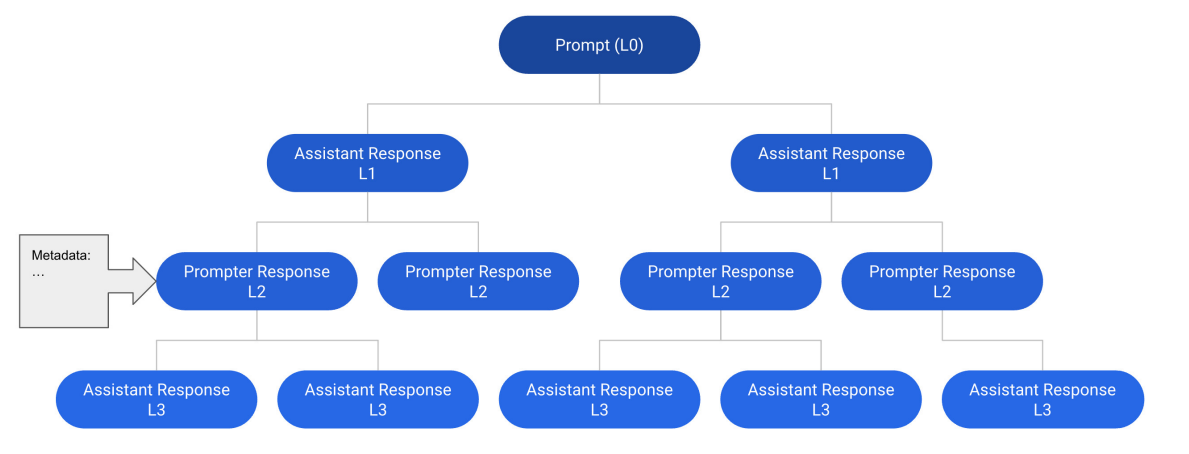
\includegraphics[width=\linewidth]{fig/dataset.png}
	\caption{\textbf{Dataset Structure} An example of a conversation tree. All paths from the root node to the leaf prompts represent unique conversations. Additionaly any two subsequent prompt and reply levels may also be used as training examples. \textit{Figure taken from the original paper by Köpf and Kilcher et. al \cite{köpf2023openassistant}}}
	\label{fig:dataset}
\end{figure}


%------------------------------------------------
\section*{Methods}

    %-------------------------
    \subsection*{Translation}
    
    With the release of the OpenAssistant Conversations Dataset (OASST1) a large open-source corpus for conversational agent finetuning is now available.
    We focus on translating the dataset in the conversation tree form where multiple replies can be nested to form conversations.
    We select a subset of trees that are ``ready for export'' as they have deleted spam messages and do not contain low quality messages and trees with only one prompt.
    Since OASST1 contains messages in various languages we translated the messages only from the 4 most common langauges in the dataset: namely English, Spanish, Russian and German.
    
    We construct pipelines for translation using NLLB-200 \cite{nllb2022} and GoogleTranslate \cite{google-translate} using the deep translator python library \cite{deep_transaltor}.
    Some of the messages also contain code which was replaced with a predefined substring at the time of translation and afterwards substituted back into the translated text.
    In this way we do not translate the code literally (eg. Translating predefined words such as \textit{import} or \textit{let}.). After initial inspection, this approach only works for code in the assistant replies as it has been nicely formated in markdown quotes  \textit{»```bash ...```«}. However when users post questions about code, they simply paste it into the prompt and thus our method of detecting code snippets was unable to detect it. 
    We decide to keep the code in the prompts translated for this version, as the target sequences are defined correctly. However, for future work developing a simple labeling model and training it on the annotated assistant responses without quotes would be a way to also detect code in the prompts.
    
    We translate 8654 trees which totals to 60,400 messages.
    We observe translations obtained using google translate are best after manual inspection. For this reason we use these as the final version of the translated dataset and leave methods for more robust translation for further work.


    %-------------------------
    \subsection*{Data Processing}
    
    We consider two possible approaches for transforming the obtained translations into features to be fed into models.
    Since some of the models are limited in the lengths of the sequences they can accept and a lot of the conversations in our conversation trees are fairly long we firstly consider splitting the conversations into pairs.
    We do this by considering each prompt and reply in a conversation and at the end filter out the pairs where the prompter was the assistant (keep only pairs where assistant is the one replying).
    
    It would also be interesting to observe the difference in not filtering out the pairs where the assistant poses the question.
    These still represent valid pairs but they are usually of the form of an answer and a follow up instruction or question.
    It's possible that such data would improve the results for general coherence of the generated sequences but not answer the question perform instructions as well.
    For training we define the prefix ``\textit{Uporabnik: }'' for all of the input prompts, while the replies do not have a specified prefix.
    We also tried training for 1 epoch with no prefixes or prefixed both of the sequences and the results were very similar. We decide to use the prefix as the model with a larger context will need prefixes to discern between assistant and user messages.
    Since one prompt can have multiple replies we end up with training examples that have the same input (prompt) sequence but a different output (reply) sequence.
    We believe that this should not be a problem and could even contribute positively since in reality there can be multiple ``correct'' replies to the same prompt.
    In this way the models will hopefully learn multiple ways to respond to a prompt and we have more examples on which the model can learn how to formulate coherent sentences.

    
    Another approach we considered is to generate all of the conversations and sub-conversations in the tree.
    This should also include all of the pairs as described above.
    We split this conversations into input and output sequences by taking the last response in the conversation as the output sequence and everything else as the input.
    In the case that the input sequence is too long for the model we only consider the end of it.
    All of the prompts and replies have the prefixes ``\textit{UPORABNIK: }'' or ``\textit{ASISTENT: }'' appended to them before the input sequence is constructed.
    Such data would be better for a larger model that can accept longer lengths and is capable of learning on more complex data.

    As we are training sequence to sequence models we only need to tokenize the above described data without the need to perform any additional feature extraction.
    However we do have some additional information/features in the metadata of the translated dataset but we mostly ignore them except for the rank. We use the rank annotations to train a model for rank response with human feedback training (RRHF~\cite{yuan2023rrhf}).


    Table \ref{tab:corpus} shows the size of our dataset and the train, validation and test splits that we created.
    We split the data with an 80-10-10 split on a shuffled dataset of conversation trees and only after process the data in a way that our models can accept.
    The ratio of the splits on the processed data is about the same as on the initially split conversation trees as we have a large enough dataset.
    

    \begin{table}[!h]
        \centering
        \scalebox{1}{
        \begin{tabular}{| l | r | r | r |r |}
            \hline
               Data Type       & Train & Val & Test & Total \\
               \hline
               Conversation Trees & 6923 & 865 & 866 & 8,654 \\
               Messages     & 60,400 & 7,554 & 7,759 & 75,713 \\
               Unique Prompts & 14,342 & 1,775 & 1,856 & 17,973 \\
               % \hline
               % \multicolumn{5}{|c|}{Prompt Reply Conversational Pairs} \\
               \hline
               Prompt - Reply & 37,902 & 4,737 & 4,875 & 47,514 \\
               Context - Reply & 54,836 & 6,874 & 7,140 & 68,850 \\
               \hline
       \end{tabular}
       }
       \caption{\textbf{Corpus Description}: This table shows the size and composition of the dataset used to train and evaluate our conversational agent.}
       \label{tab:corpus}
    \end{table}

    We make the current version of the dataset publicly available on Kaggle \url{https://www.kaggle.com/datasets/valterh/oasst1-sl}. As well as all of the trained models.

    %-------------------------
    \subsection*{Model Training}
    We train 5 conversational models on the context-answer and prompt-answer datasets as a way to asses the suitability of the dataset for conversational agent training. 
    We train T5 variants and GPT-2 as well as a SloBerta model for reply ranking.
    \subsubsection*{Conversational Models}
    \noindent\textbf{T5} We fine-tune a T5-small model on answer pairs and two T5 large models. During the training of the large versions our training code kept crashing after the first epoch and thus we fit these models only for a sinlge epoch. Despite this these models still produce the best results out of all the trained models.
    
    \noindent\textbf{GPT} We fine-tune two gpt-sl-base models for 10 epochs, one on context answers and one on prompt answer pairs. The training loss is visualized in  Fig.~\ref{fig:training}.


    \subsubsection*{Rank Response Alignment}
    
    \noindent\textbf{RRHF - SloBerta}
    We train a Sloberta pretrained sentence classification model. We define the ranking as a classification task, where the model must classify a prompt-response pair into one of five ordinal categories as annotated in the dataset. The model does not converge well and we see little improvement with adoption of this method.


%------------------------------------------------

\section*{Results}

% Use the results section to present the final results of your work. Present the results in a objective and scientific fashion. Use visualisations to convey your results in a clear and efficient manner. When comparing results between various techniques use appropriate statistical methodology.

    We evaluate the models using the following metrics:
    BERTScore, a metric that evaluates text quality by comparing generated or translated text to reference text using BERT embeddings. It captures contextual information to calculate similarity, considering word and phrase matches.

    ROUGE is a set of metrics for evaluating summarization and machine translation outputs. It measures content overlap using n-gram matches and sequence-based measures, providing insights into system effectiveness.

    \begin{table*}[thb]
    	\caption{\textbf{Performance Comparison}}
    	\centering
        \scalebox{1}{
    	\begin{tabular}{c l | c c c | c c c c}
    
                   & & \multicolumn{3}{c|}{Bertscore} & \multicolumn{4}{c}{ROUGE} \\
            Epochs & Model & Precision & Recall & F1        &  rouge1 & rouge2 & rougeL & rougeLsum \\
    		\hline \hline
            /  & t5-small            & 62.46 & 44.09 & 51.45 & 0.34  & 0.06 & 0.25  & 0.31 \\
            25 & t5-small-pairs      & 66.93 & 63.37 & 64.92 & 17.23 & 4.08 & 11.48 & 15.73 \\
            \hline
            1 & t5-large-pairs       & 66.84 & 62.46 & 64.39 & 14.71 & 3.61 & 10.39 & 13.31 \\
            1 & t5-large-conv        & 72.25 & 65.86 & 68.63 & 18.00 & 4.16 & 14.16 & 16.78 \\
            \hline
            /  & GPT         & 59.51 & 62.74 & 60.97 & 15.02 & 2.44 & 9.13 & 13.54 \\
            10 & GPT-pairs   & 61.03 & 63.76 & 62.24 & 16.90 & 2.63 & 9.82 & 15.61 \\
            10 & GPT-conv    & 60.56 & 65.20 & 62.60 & 14.78 & 2.40 & 8.84 & 13.65 \\
            
    	\end{tabular}
        }
    	\label{tab:results}
    \end{table*}

    \begin{figure}[h]\centering
	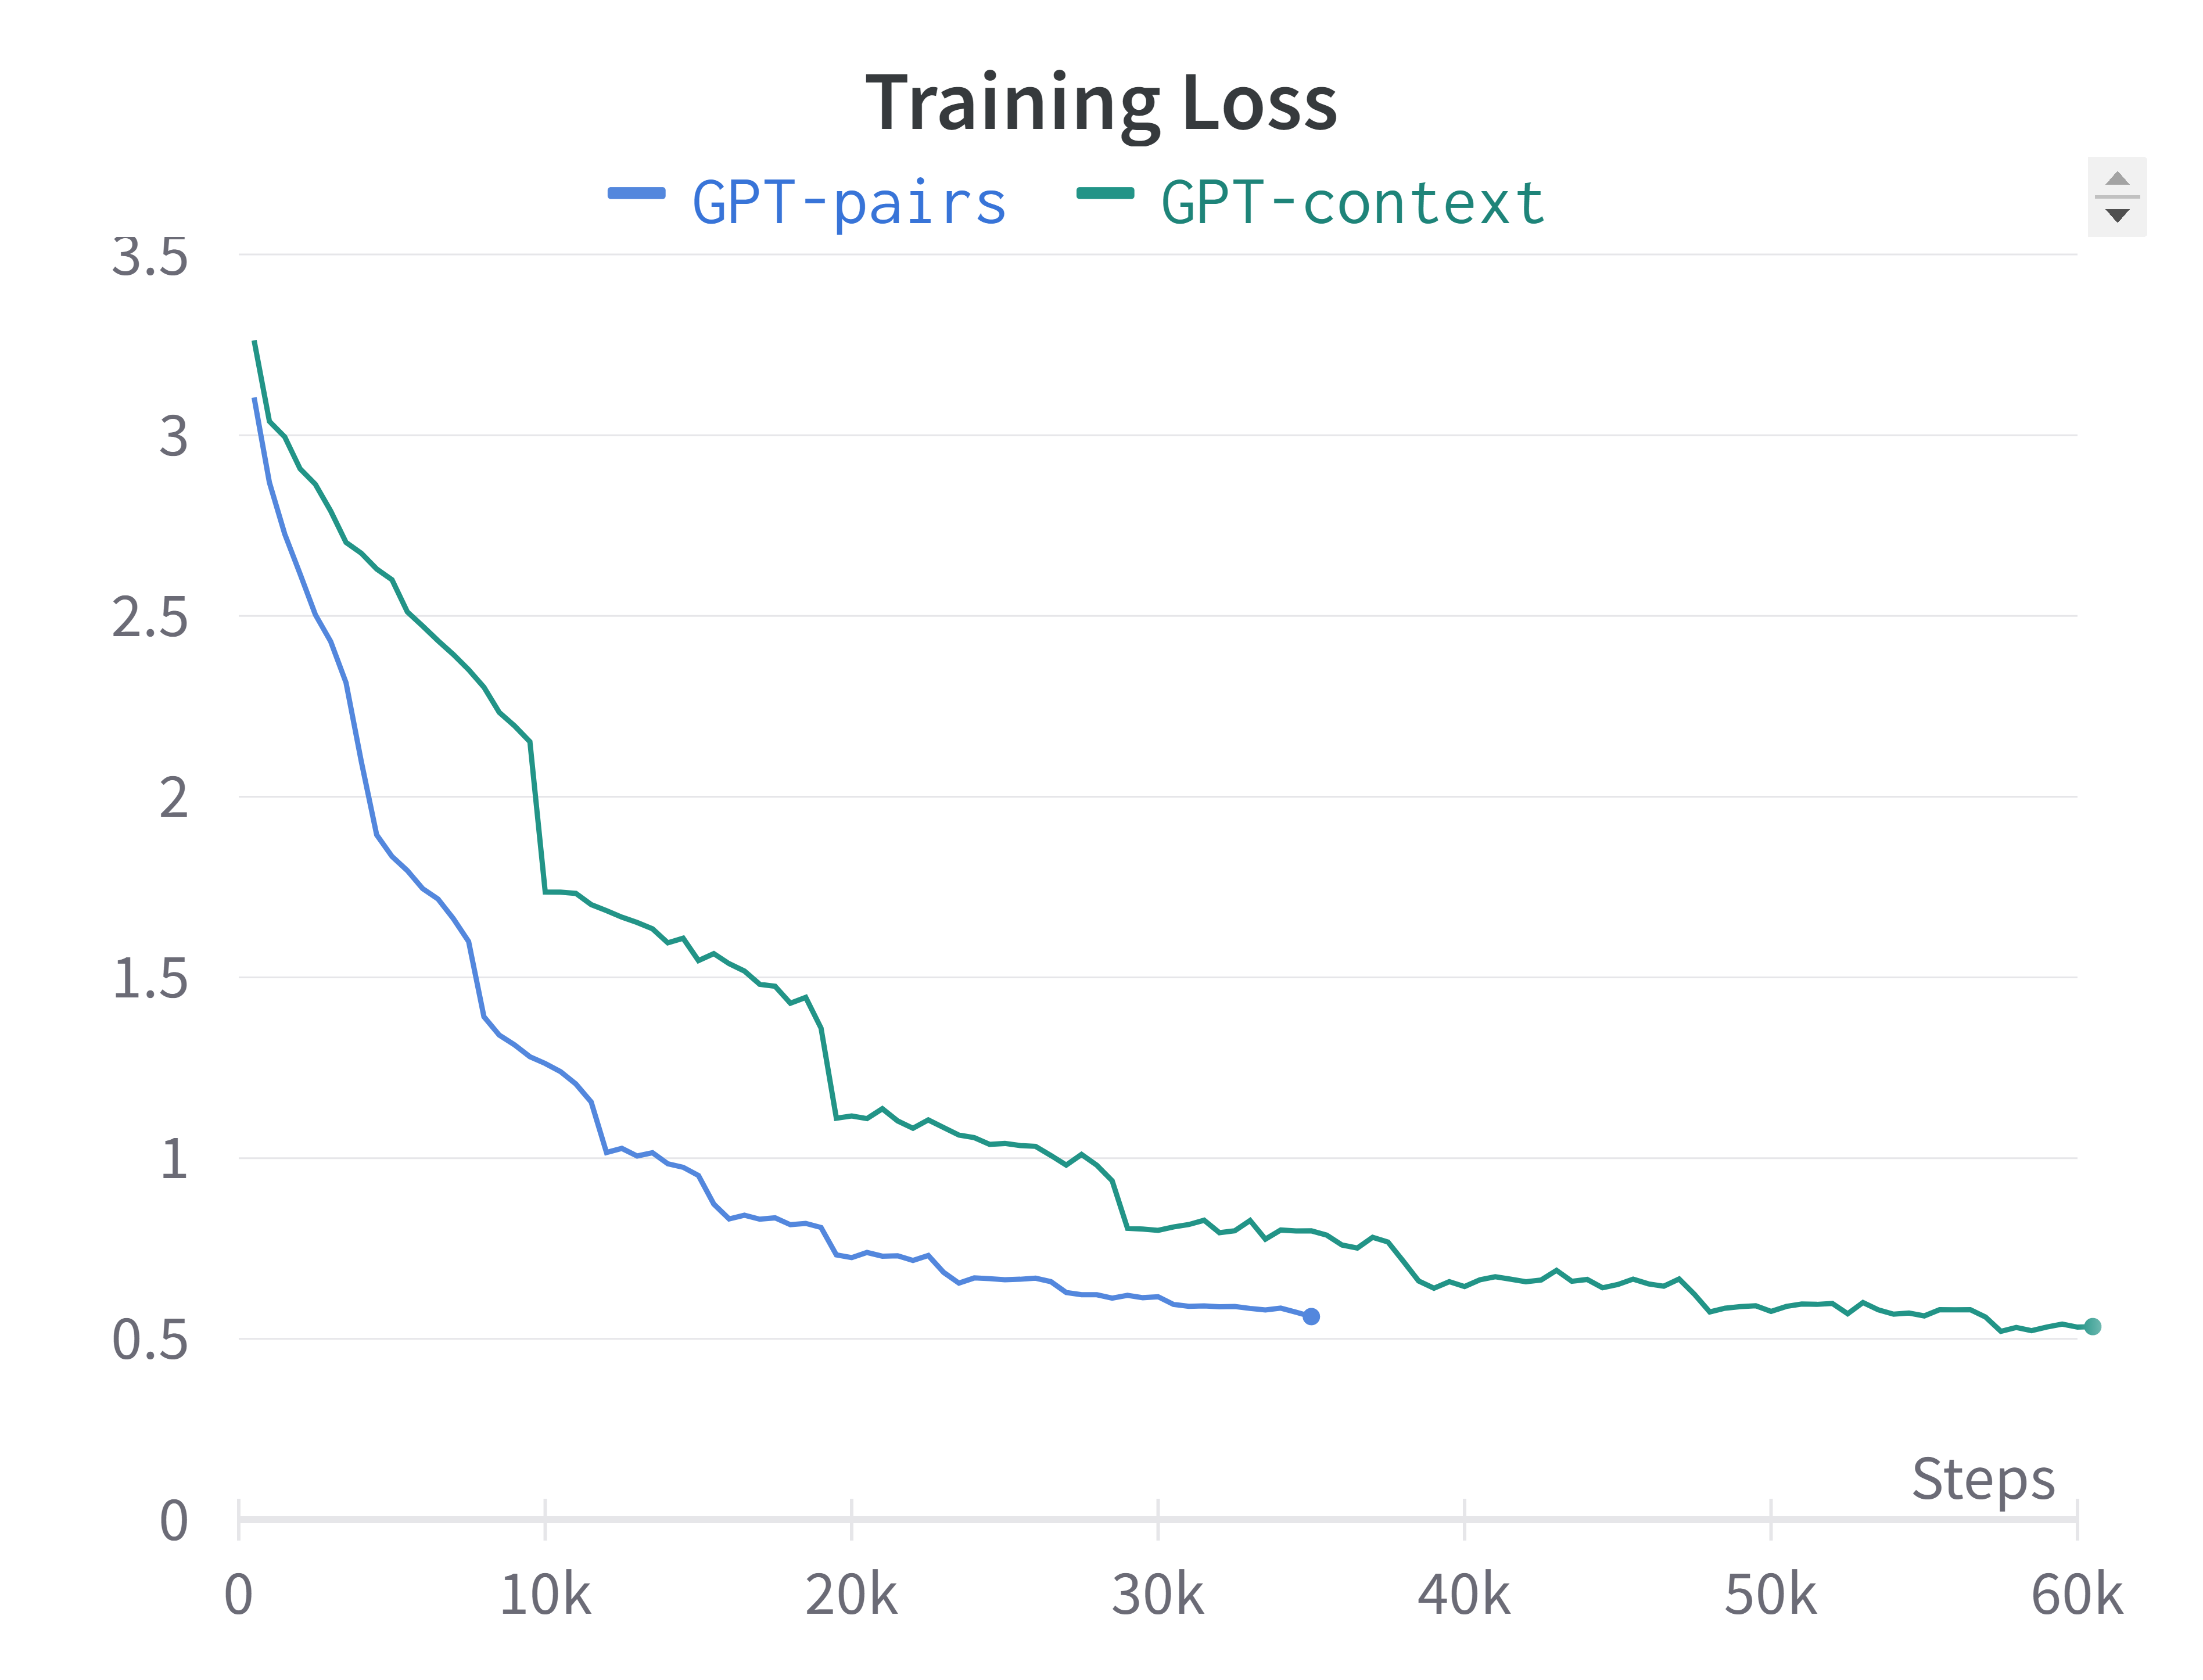
\includegraphics[width=\linewidth]{fig/training_loss.png}
	\caption{\textbf{GPT-B Training Loss.} GPT models with context and reply pairs were trained for 10 epochs each. The difference in the number of steps is due to the training set sizes.}
	\label{fig:training}
    \end{figure}

    In Table \ref{tab:results} we can observe the scores obtained using our models.
    We can see that all of the models improve in the number of epochs we left them to train (different because of limitations with computational resources and time).
    We observe that the training loss of all models quickly drops in the first few epochs and the only slightly decreases with time which can be seen in Figure~\ref{fig:training} for two of the fitted models.
    
    %-------------------------
    \subsection*{Qualitative results}
    Alongside the quantitative evaluation using the ROUGE and Bert scores we also perform qualitative evaluation. We compare the outputs of our model to the responses of ChatGPT in Slovene and OpenAssistant replies translated to Slovene.\footnote{At the time of writing Google's Bard is unavailable in Slovenia}
    Table~\ref{tab:results_qualitative} showcases a qualitative comparison of a few replies from our model (t5-small fitted on pairs), ChatGPT and Open Assistant.
    We can observe that while our model generates much shorter sequences and they are not always factually correct (the others also have some mistakes) it forms coherent replies and generally performs quite well.
    We believe that if we trained the larger model for the same amount of time we would improve the results even further and form even better sequences.
    Additional data and/or a bigger model should also benefit the results we currently observe especially in regards to the factual correctnes of replies.
    

    \begin{table*}[hbt]
    	\caption{\textbf{Qualitative Comparison to Available Conversational LLMs, uning the fine-tuned T5-Small model}}
    	\centering
        \scalebox{1}{
    	\begin{tabular}{l}
            
            \hline %\hline
            
            % PROMPT 1
            \textbf{Prompt}: Kaj je ljubezen? \\
            \hline
            
            \textbf{Ours}: Ljubezen je čustvo, ki se nanaša na odnos med dvema osebama.
            \vspace{2.5px} \\
            
            \textbf{ChatGPT}: Ljubezen je kompleksen in globok čustveni občutek, ki se lahko manifestira na različne načine.\\ Ljubezen je lahko občutek globoke naklonjenosti, strasti, privrženosti ali predanosti do nekoga ali nečesa. Prav tako\\ se lahko ljubezen izraža skozi dejanja, skrb, sočutje in sprejemanje...
            
            \vspace{2.5px}\\
            
            \textbf{Open Assistant}: Ljubezen je čustvo, ki ga ne more opisati v besedah. Vključuje različne oblike \\uživanja in strasti ter predstavlja široko paleto intenzivnih doživetij. Po navadi jo povezujemo z osjećanjem strasti\\ ali pripadnosti, na primer kjer se dvema osebama spodbuja sredstvo komuniciranja, npr. videz, glas, notranji duh itd... \\Pri tem lahko pride do tranzu. \\
            
            
            % PROMPT 2
            \\
            \hline %\hline
            \textbf{Prompt}: Kdo je France Prešeren? \\
            \hline
            \vspace{2.5px}
            \textbf{Ours}: France Prešeren je bil francoski pesnik, ki se je rodil leta 1922 v Parizu.
            \vspace{2.5px} \\
            
            \textbf{ChatGPT}: France Prešeren je bil slovenski pesnik, ki je živel med letoma 1800 in 1849. Velja za\\ najpomembnejšega slovenskega pesnika in nacionalnega junaka. Prešeren je pomembno vplival na razvoj slovenske\\ književnosti in slovenskega narodnega zavedanja.
            Njegovo najbolj znano delo je pesnitev "Zdravljica", ki je pozneje postala\\ slovenska himna. Prešeren je ustvarjal v romantiki in njegova poezija se odlikuje po bogati simboliki, globokih čustvih,\\ pesimizmu in iskanju svobode. Njegovi pesniški motivi so ljubezen, narava, patria in sočutje do človeka. France Prešeren\\ je prejel številna priznanja za svoje delo, vključno z nazivom največjega slovenskega pesnika. Njegov rojstni dan,\\3. december, je v Sloveniji tudi državni praznik, imenovan Prešernov dan, ko se praznuje slovenska kultura in umetnost.
            \vspace{2.5px} \\
            
            \textbf{Open Assistant}: France Prešeren je bil slovenski pesnik in pravnik. Velja za enega največjih slovenskih romantičnih\\ pesnikov, najbolj znan po svoji liriki, ki jo je pisal v 19. stoletju. Njegova najbolj znana pesem se imenuje Zdravljica,\\ ki je postala slovenska himna...

            % PROMPT 3
            \\
            \hline %\hline
            \textbf{Prompt}: Kdo velja za najboljšega nogometaša? \\
            \hline
            
            \textbf{Ours}: Najboljši nogometaš, ki velja za najboljšega nogometaša na svetu, je Cristiano Ronaldo.
            \vspace{2.5px} \\
            
            \textbf{ChatGPT}: Kot je moj znanje trenutno posodobljeno do septembra 2021, najboljši nogometaši so se skozi zgodovino\\ spreminjali in ocenjevali na različne načine. Obstaja več pomembnih nagrad in priznanj, ki se podeljujejo za dosežke v\\ nogometu, kot so Zlata žoga (FIFA), FIFA The Best, UEFA igralec leta, PFA igralec leta itd...
            \vspace{2.5px} \\
            
            \textbf{Open Assistant}: Lionel Messi velja za najboljšega argentinskega nogometaša. Messi, ki je vrsto let igral za FC Barcelono,\\ preden se je pridružil Paris Saint-Germainu (PSG), je prejel številne individualne nagrade, vključno z več naslovi FIFA\\ Ballon d'Or. Njegove izjemne sposobnosti, agilnost, vizija in sposobnost doseganja golov so mu prislužile sloves enega\\ najboljših nogometašev vseh časov.

            
            
    	\end{tabular}
        }
    	\label{tab:results_qualitative}
    \end{table*}

%------------------------------------------------

\section*{Discussion}
    The results of the models tell us that it is important to correctly define the finetuning process. Different models behave differently, and thus when they are trained on the same dataset, we can expect different performance. This is only exasperated by the fact that they were not trained equally. While it is made sure that they are trained with the same hyper-parameters, the available hardware, made it difficult to finetune all the models for the same amount of time. This shortcoming, makes it difficult to directly compare the models, and while we can infer to the true behaviour, we can't draw direct comparisons.\\
    During the RRHF inference we should be able to produce multiple replies using our finetuned language model and then employ reply ranking to select the best reply. However, because the model does not fit well (has oscillating loss), this process produces almost the same probabilities every time. We conclude, that more care should be taken to better fit the model, which could produce better results.   

% Results and discussion show the results and comments on the performance of algorithms. Discussion also points out where the algorithms do not work well and where they achieve good performance. In the conclusion the authors should point out shortcomings of their approaches and give at least one idea for improvements in the future. When reading the report, you could get a feeling that authors know what they are doing, sensibly selected approaches and critically explain and discuss their results.

% Use the Discussion section to objectively evaluate your work, do not just put praise on everything you did, be critical and exposes flaws and weaknesses of your solution. You can also explain what you would do differently if you would be able to start again and what upgrades could be done on the project in the future.

    %-------------------------
    \subsection*{Future work}
    % FURTHER WORK
    % Plan for enriching dataset
    For future work, combining translations from multiple sources and back-translation could improve the consistency and coherence of the conversational data.
    
    Furthermore, conducting manual inspection to identify specific linguistic nuances and subtle information that may have been lost in the translation process. This involves closely examining the messages for wordplay, understanding error messages, and capturing the underlying semantics accurately. 
    Additionally, we will explore the transformation of message formality by applying lemmatization techniques. By changing the prompts from a more formal style to an informal and conversational tone, we aim to create a dataset that better aligns with natural language interactions and user preferences.
    
    These future research directions will contribute to the refinement and enhancement of translated datasets, facilitating improved performance and user experiences in multilingual conversational applications especially for few resource languages such as Slovene.
    
    The assistant could be further improved upon by using an even larger model. An example of this would be the 7 billion parameter LLaMA model. However, since LLaMA does not inherently support Slovenian (it only supports English, Spanish, French, German, Italian, Portuguese, and Dutch), additional pretraining on Slovenian corpora should be considered. The most important among these being Gigafida~\cite{11356/1320} and ccKRES~\cite{ccKres}, but we could also consider GOS~\cite{Verdonik2013} to cover spoken language and the Šolar corpus \cite{kosem2011slovenian}, with considerations that the written language of primary and high school students could potentially increase the models performance.


%------------------------------------------------

\section*{Conclusion}
 In summary, our project aims to develop a Slovenian Conversational Agent, by leveraging large language models, transformers, and the OpenAssistant Conversations dataset. Through translation, data processing, and appropriate training, we show that a coherent conversational agent may be trained even for a low resource language. With additional pre-training and a larger architecture this dataset has the potential for a true Slovenian Large Language Model.

%------------------------------------------------

% \section*{Acknowledgments}

% Here you can thank other persons (advisors, colleagues ...) that contributed to the successful completion of your project.


\clearpage
%----------------------------------------------------------------------------------------
%	REFERENCE LIST
%----------------------------------------------------------------------------------------
\bibliographystyle{unsrt}
\bibliography{report}


\end{document}